\documentclass[tikz, margin=1mm]{standalone}
\usetikzlibrary{calc}

\begin{document}
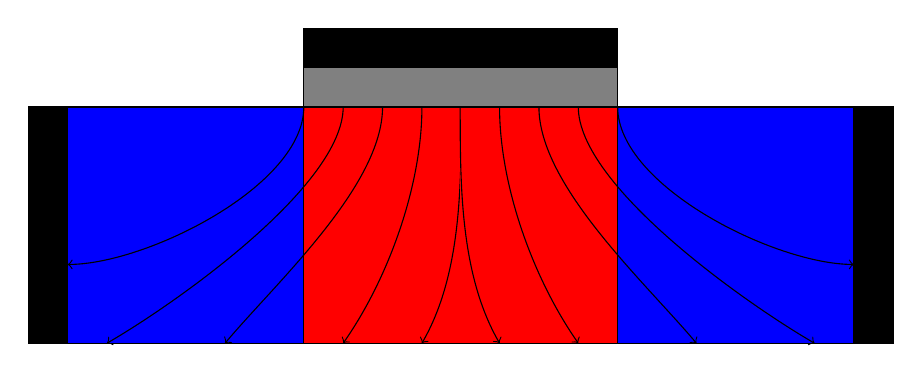
\begin{tikzpicture}

\def\do{
\draw[fill=black] (-5, 0) -- (-5, -3) -- (-5.5, -3) -- (-5.5, 0) -- cycle;
\draw[fill=blue] (-5, 0) -- (-5, -3) -- (-2, -3) -- (-2, 0) -- cycle;
\fill[red] (-2, 0) -- (-2, -3) -- (0, -3) -- (0, 0) -- cycle;
%
\fill[gray] (-2,0) rectangle (0, .5);
\draw (0,0) -- (-2,0) -- (-2,-3) -- (0, -3);
\draw (-2,0.5) -- (-2,0);
\draw[fill=black] (-2, .5) rectangle (0, 1); 
%
% see TikZ manual for special interpretation of relative coordinates for Bezier curves
% on-state (electrons attracted to n-p interface in npn transistor)
\draw[->] (0, 0) .. controls +(270:1cm) and +(60:1cm) .. (-0.5,-3);
\draw[->] (-0.5,0) .. controls +(270:1cm) and +(55:1cm) .. (-1.5,-3);
\draw[->] (-1,0) .. controls +(270:1cm) and +(50:1cm) .. (-3,-3);
\draw[->] (-1.5,0) .. controls +(270:1cm) and +(30:1cm) .. (-4.5,-3);
\draw[->] (-2,0) .. controls +(270:1cm) and +(0:1cm) .. (-5,-2);
% off-state (electrons not attracted to n-p interface in npn transistor)
%\draw[<-] (0, 0) .. controls +(270:1cm) and +(60:1cm) .. (-0.5,-5);
%\draw[<-] (-0.5,0) .. controls +(270:1cm) and +(55:1cm) .. (-1.5,-5);
%\draw[<-] (-1,0) .. controls +(270:1cm) and +(50:1cm) .. (-3,-5);
%\draw[<-] (-1.5,0) .. controls +(270:1cm) and +(45:1cm) .. (-4.5,-5);
%\draw[<-] (-2,0) .. controls +(270:1cm) and +(40:1cm) .. (-6,-5);
}
%
\do
%
\begin{scope}[xscale=-1,xshift=.4pt] % linewidth
\do
\end{scope}
\end{tikzpicture}
\end{document}
